\documentclass[a4paper,12pt]{article}

% ----------------------------
% Pacchetti utili
% ----------------------------
\usepackage[utf8]{inputenc}
\usepackage[T1]{fontenc}
\usepackage[italian]{babel}
\usepackage{graphicx}
\usepackage{tabularx}
\usepackage[table]{xcolor}
\definecolor{lightblue}{RGB}{225,240,255}
\definecolor{gold}{RGB}{255,215,0}
\usepackage{geometry}
\usepackage{setspace}
\usepackage{calc}
\usepackage{array}
\usepackage{fancyhdr}
\usepackage{comment}
\usepackage{tikz}
\usepackage{float}
\usepackage{amsmath}
\usepackage{pgf-pie}
\usepackage{longtable}
\usepackage[colorlinks=true, linkcolor=blue, urlcolor=blue, citecolor=blue]{hyperref}
\usepackage{pgffor}

% ----------------------------
% Impostazioni pagina
% ----------------------------
\geometry{
    top=2cm,
    bottom=2cm,
    left=2cm,
    right=2cm
}

\setstretch{1.2}

% ----------------------------
% Dati personalizzabili
% ----------------------------
\newcommand{\Gruppo}{Atlas}
\newcommand{\Email}{\href{mailto:team9.atlas@gmail.com}{\textcolor{blue}{\underline{team9.atlas@gmail.com}}}}
\newcommand{\TitoloDocumento}{Manuale Utente}
\newcommand{\DataUltimaModifica}{2026/04/08}
\newcommand{\LogoGruppo}{../../../Assets/AtlasLogo.png}

% --- Nuove variabili aggiunte ---
\newcommand{\VersioneDocumento}{v1.0.0}
\newcommand{\TipoDocumento}{Esterno} 

\pagestyle{fancy}
\fancyhf{}
\fancyhead[L]{\Gruppo}
\fancyhead[R]{Documento: \TipoDocumento}
\fancyfoot[C]{\thepage}

% larghezza della colonna dei nomi
\newlength{\namecol}
\setlength{\namecol}{4.5cm}
\setlength{\headheight}{15pt} % messo per evitare warning di fancyhdr


\newlength{\colw}
\setlength{\colw}{1.5cm}

\setcounter{secnumdepth}{5}
\setcounter{tocdepth}{5}

\definecolor{mioverde}{RGB}{20,150,60}

% ----------------------------
% Inizio documento
% ----------------------------
\begin{document}

% ----------------------------
% Prima pagina
% ----------------------------
\begin{titlepage}

    \begin{center}

        % Logo
        \vspace*{0cm}
        \begin{tikzpicture}
            \clip (0,-0.1) circle (5.6cm);
            \node at (0,0) {\includegraphics[width=12cm]{\LogoGruppo}};
        \end{tikzpicture}\\[0.8cm]

        % Barra superiore
        \noindent\rule{\textwidth}{0.4pt}

        % Titolo
        \vspace{1cm}
        {\Huge \textbf{\TitoloDocumento}}\\[0.4cm]
        {\large Progetto di Ingegneria del Software A.A. 2025/2026}\\[0.8cm]
        {\large Versione: \VersioneDocumento}
        \vspace{1cm}

        % Barra inferiore
        \noindent\rule{\textwidth}{0.4pt}

    \end{center}

    % Informazioni in basso
    \vfill
    \noindent
    \begin{minipage}{0.5\textwidth}
        \raggedright
        \textbf{Autore:} \Gruppo\\
        \textbf{Ultima modifica:} \DataUltimaModifica
    \end{minipage}%
    \begin{minipage}{0.5\textwidth}
        \raggedleft
        \textbf{Tipo di documento:} \TipoDocumento
    \end{minipage}

\end{titlepage}



\section*{Registro delle modifiche}
\begin{center}
    \rowcolors{2}{lightblue}{white}
    \begin{tabularx}{\textwidth}{|l|l|l|X|X|}
        \hline
        \rowcolor{lightgray}
        \textbf{Versione}  & \textbf{Data}       & \textbf{Autore}      & \textbf{Verificatore} & \textbf{Descrizione}  \\
        \hline
        \VersioneDocumento & \DataUltimaModifica & Giacomo Giora & Michele Tesser & Aggiunte g del Glossario v2.0.0. Ricevuta approvazione \\
        \hline
        v0.5.1 & 2026/04/03 & Bilal Sabic & Michele Tesser & Fine stesura \newline documento \\
        \hline
        v0.5.0 & 2026/03/31 & Bilal Sabic & Michele Tesser & Sistemazione contenuti \\
        \hline
        v0.4.0 & 2026/03/30 & Bilal Sabic & Michele Tesser & Aggiunta sezione \newline errori \\
        \hline
        v0.3.0 & 2026/03/27 & Bilal Sabic & Michele Tesser & Aggiunte foto \\
        \hline
        v0.2.0 & 2026/03/26 & Bilal Sabic & Michele Tesser & Aggiunta sezione \newline requisiti \\
        \hline
        v0.1.0 & 2026/03/15 & Bilal Sabic & Federico Simonetto & Prima stesura \newline documento \\
        \hline
    \end{tabularx}
\end{center}

\newpage

\tableofcontents

\newpage

\listoffigures

%\newpage

%\listoftables

\newpage

\section{Introduzione}

    \subsection{Scopo del documento}
        Il presente documento ha l'\textit{obiettivo}\textsubscript{\href{https://atlasteam9.github.io/Atlas/glossario.html\#Obiettivo}{G}} di fornire una guida all'utilizzo dell'applicazione sviluppata dal team \textit{Atlas}, realizzata su richiesta del proponente \textit{Bluewind S.r.l.} nell'ambito del \textit{capitolato}\textsubscript{\href{https://atlasteam9.github.io/Atlas/glossario.html\#Capitolato}{G}} \textbf{C1 - Automated EN18031 Compliance Verification}. \newline
        Il documento è finalizzato a supportare l'utente finale nelle fasi di installazione e di utilizzo dell'applicazione software. A tal fine vengono descritti i requisiti hardware e software necessari, nonché le procedure da seguire per l'installazione e per il corretto utilizzo del sistema.

    \subsection{Scopo del prodotto}
        L'\textit{obiettivo}\textsubscript{\href{https://atlasteam9.github.io/Atlas/glossario.html\#Obiettivo}{G}} del prodotto è automatizzare il processo di verifica della conformità degli apparecchi che utilizzano onde radio rispetto alla normativa europea EN18031, definita dalla Direttiva RED. \newline
        L'applicazione sviluppata consente di effettuare tale verifica tramite l'esecuzione di specifici \textit{decision tree} associati ai diversi asset del dispositivo. Al termine dell'esecuzione, il sistema fornisce un risultato chiaro della valutazione, espresso attraverso uno dei seguenti esiti: \textit{PASS}, \textit{FAIL} oppure \textit{NOT APPLICABLE}.

    \subsection{Contesto d'uso}
        Come già esplicitato nel documento \href{https://atlasteam9.github.io/Atlas/docs/PB/documenti/esterni/Analisi%20dei%20Requisiti.pdf}{Analisi dei Requisiti v2.0.0}, gli utenti finali dell'applicazione \textbf{Automated EN18031 Compliance Verification} appartengono alla categoria degli "utenti esperti". Essi possiedono pertanto competenze tecniche in ambito di \textit{sicurezza informatica}\textsubscript{\href{https://atlasteam9.github.io/Atlas/glossario.html\#Sicurezzainformatica}{G}} e conoscenze della normativa europea a cui il \textit{capitolato}\textsubscript{\href{https://atlasteam9.github.io/Atlas/glossario.html\#Capitolato}{G}} fa riferimento. \newline
        Per tale motivo, nel presente documento viene fatto deliberatamente uso di terminologia tecnica.

    \subsection{Glossario}
        All'interno della documentazione prodotta dal team possono comparire termini suscettibili di incomprensioni o ambiguità. Per evitare questo, è disponibile un glossario
        contenente i termini tecnici e le loro definizioni. Un termine è consultabile nel glossario se è indicato con la notazione \textit{parola\textsubscript{\href{https://atlasteam9.github.io/Atlas/glossario.html}{G}}}.
        Premendo sulla G a pedice, l'utente verrà indirizzato alla pagina web del \textit{Glossario v.2.0.0}.
    

    \subsection{Riferimenti}
        \subsubsection{Riferimenti normativi}
            \begin{itemize}
                \item Riferimento al \textit{capitolato}\textsubscript{\href{https://atlasteam9.github.io/Atlas/glossario.html\#Capitolato}{G}} 1 dell'azienda proponente:\newline \textbf{Bluewind S.r.l - Automated EN18031 Compliance Verification}\newline \url{https://www.math.unipd.it/~tullio/IS-1/2025/Progetto/C1.pdf}
                \item Riferimento al Way of Working del team Atlas: \newline \textbf{Norme di Progetto v.2.0.0}\newline \href{https://atlasteam9.github.io/Atlas/docs/PB/documenti/interni/Norme%20di%20Progetto.pdf}{Link al documento} 
            \end{itemize}

\newpage
\section{Requisiti}
    \subsection{Requisiti hardware}
        Qui vengono elencati tutti i requisiti hardware minimi per ogni componente dell'applicazione:
        \begin{center}
            \rowcolors{2}{lightblue}{white}
            \begin{tabularx}{\textwidth}{|l|l|l|l|X|}
                \hline
                \rowcolor{gold} 
                \textbf{Componente}  & \textbf{RAM}  & \textbf{CPU}     & \textbf{Memoria}    
                & \textbf{Sistema \newline operativo}   \\
                \hline
                \textbf{Docker} & {4GB} &  {64-bit con virtualizzazione} & 10-20GB & {Windows 10 64-bit, macOS 11, Linux} \\
                \hline
                \textbf{Git} & {512MB} & {Qualsiasi CPU moderna} & {200MB} & {Windows 7, macOS 10, Linux} \\
                \hline
                \textbf{Google Chrome} & {4GB} & {Pentium 4} & {500MB} & {Windows 10, \newline macOS 11, Linux} \\
                \hline
                \textbf{Mozilla Firefox} & {2GB} & {1GHz o più veloce} & {300MB} & {Windows 10, \newline macOS 10, Linux}\\
                \hline
                 \end{tabularx}
                 \end{center}
                 Sono stati elencati sia Chrome che Firefox perché sono i due browser più utilizzati. 
                 Tutti i componenti si possono scaricare dai loro siti dedicati. \newline
                 Per garantire una buona esperienza d'uso, si raccomanda che il sistema soddisfi i seguenti requisiti  hardware minimi.
        \begin{center}
        \rowcolors{2}{lightblue}{white}
            \begin{tabularx}{\textwidth}{|l|l|l|X|}
                \hline
                \rowcolor{gold} 
                \textbf{RAM}  & \textbf{CPU}  & \textbf{Memoria}  & \textbf{Sistema operativo}   \\
                \hline
                {4GB} & {64-bit con supporto per la virtualizzazione} & {10-20GB} & {Windows 10 64-bit,  \newline macOS 11, Linux} \\
                \hline
        \end{tabularx}
        \end{center}
                 
    \subsection{Requisiti software}
        L'applicazione richiede l'installazione dei seguenti software:
        \begin{itemize}
            \item \textbf{Docker Engine} (Linux) o \textbf{Docker Desktop} (Windows, Mac);
            \item \textbf{Git (opzionale)}.
        \end{itemize}

        Il prodotto software viene distribuito tramite container \textit{Docker}\textsubscript{\href{https://atlasteam9.github.io/Atlas/glossario.html\#Docker}{G}}; pertanto non è necessario installare librerie o \textit{servizi}\textsubscript{\href{https://atlasteam9.github.io/Atlas/glossario.html\#Servizi}{G}} di supporto aggiuntivi. \newline
        \textbf{Docker}, infatti, consente di eseguire l'applicazione all'interno di un container, garantendo un ambiente di esecuzione isolato e configurato correttamente.
        \textbf{Git} viene utilizzato per clonare la \textit{repository}\textsubscript{\href{https://atlasteam9.github.io/Atlas/glossario.html\#Repository}{G}} \textit{GitHub}\textsubscript{\href{https://atlasteam9.github.io/Atlas/glossario.html\#GitHub}{G}} contenente il progetto, ma è altrettanto possibile scaricare il prodotto in formato .zip tramite il sito del team \href{https://atlasteam9.github.io/Atlas/}{Atlas}.
\newpage

\section{Installazione}
    \subsection{Installazione di Docker}    
        Prima di procedere con l'installazione dell'applicazione bisogna verificare che \textit{Docker}\textsubscript{\href{https://atlasteam9.github.io/Atlas/glossario.html\#Docker}{G}} sia presente sulla propria macchina. Per farlo, si digita nel terminale: \newline 
        \textbf{docker --version}\newline
        Se la console ritorna una versione di \textit{Docker}\textsubscript{\href{https://atlasteam9.github.io/Atlas/glossario.html\#Docker}{G}}, ad \textit{esempio}\textsubscript{\href{https://atlasteam9.github.io/Atlas/glossario.html\#Esempio}{G}}: "\textbf{Docker version 28.5.2, build ecc6942}",
        allora \textit{docker}\textsubscript{\href{https://atlasteam9.github.io/Atlas/glossario.html\#Docker}{G}} è correttamente installato. Se invece ritorna un \textit{errore}\textsubscript{\href{https://atlasteam9.github.io/Atlas/glossario.html\#Errore}{G}}, è possibile scaricarlo dal seguente sito \url{https://docs.docker.com/engine/install/} seguendo la guida. Durante lo \textit{sviluppo}\textsubscript{\href{https://atlasteam9.github.io/Atlas/glossario.html\#Sviluppo}{G}} dell'applicazione è stata utilizzata la versione 29.3.0 di Docker.
        \subsection{Download dell'applicazione}
        Il download si può effettuare in due modi:
        \begin{itemize}
        \item \textit{Git}\textsubscript{\href{https://atlasteam9.github.io/Atlas/glossario.html\#Git}{G}}: è possibile clonare la \textit{repository}\textsubscript{\href{https://atlasteam9.github.io/Atlas/glossario.html\#Repository}{G}} di \textit{GitHub}\textsubscript{\href{https://atlasteam9.github.io/Atlas/glossario.html\#GitHub}{G}} eseguendo nel terminale \newline \textbf{git clone https://github.com/AtlasTeam9/MVP}
        \item da browser: andare sul sito della \href{https://github.com/AtlasTeam9/MVP}{\textit{repository}\textsubscript{\href{https://atlasteam9.github.io/Atlas/glossario.html\#Repository}{G}}} e scaricare la repo in formato .zip
        \end{itemize}
        Una volta scaricato, posizionarsi nella cartella "MVP-main".

        \subsection{Creazione dell'immagine e l'avvio del container}
        Dopo essersi posizionati nella cartella principale, digitare nel terminale: 
        \begin{itemize}
          \item \textbf{cp .env.example .env} (solo la prima volta)
          \item \textbf{docker compose up --build}
        \end{itemize}
        La creazione dell'immagine richiede pochi minuti (circa 1-2). Dopo il processo di creazione viene costruito ed avviato il container della web-app. Per chiudere la sessione di \textit{Docker}\textsubscript{\href{https://atlasteam9.github.io/Atlas/glossario.html\#Docker}{G}} basta inserire la combinazione di tasti Ctrl+C, oppure premere il tasto stop che si trova nella sezione actions se si utilizza \textit{Docker}\textsubscript{\href{https://atlasteam9.github.io/Atlas/glossario.html\#Docker}{G}} Desktop. \newline Se si vuole riprendere la sessione di \textit{Docker}\textsubscript{\href{https://atlasteam9.github.io/Atlas/glossario.html\#Docker}{G}} si può fare digitando nel terminale:
        \begin{itemize}
          \item \textbf{docker compose up} 
        \end{itemize}
        Si può sempre chiudere premendo Ctrl+C oppure premendo stop.
        
        \subsection{Esecuzione della web-app}
        Dopo aver seguito tutti i passi precedenti, aprire un browser e scrivere nella barra di ricerca:
        \begin{itemize}
          \item \textbf{localhost:8080}
        \end{itemize}
        Si aprirà l'\textit{interfaccia}\textsubscript{\href{https://atlasteam9.github.io/Atlas/glossario.html\#Interfaccia}{G}} dell'applicazione web, pronta per l'uso. Nella seguente sezione si trovano le istruzioni per l'utilizzo della web-app.
        
\newpage

\section{Istruzioni per l'uso}
    Questa sezione descrive le principali azioni che si possono svolgere all'interno dell'applicazione.
    \subsection{Homepage}
    L'\textit{interfaccia}\textsubscript{\href{https://atlasteam9.github.io/Atlas/glossario.html\#Interfaccia}{G}} principale della web-app. Sono presenti 3 pulsanti: Upload Device(JSON), Create New Device, Upload Previous Session.
    \begin{center}
        \begin{figure}[H]
              \centering
              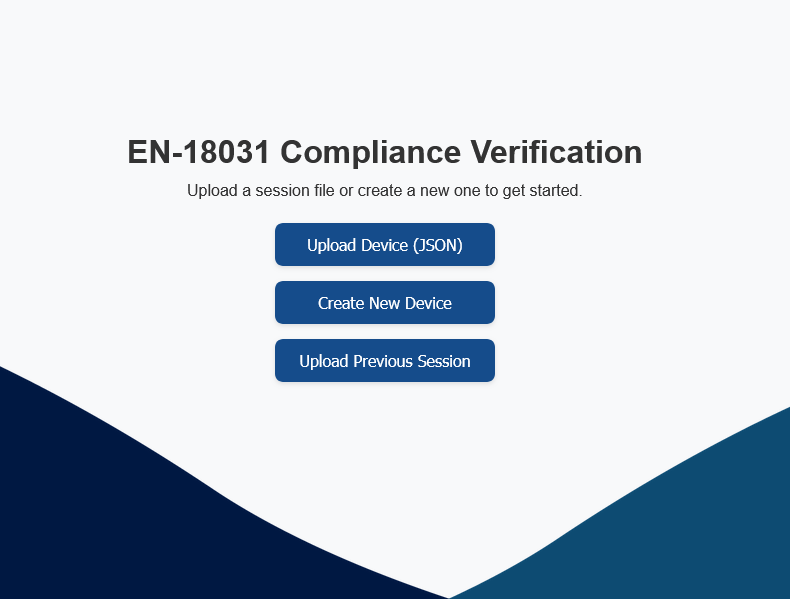
\includegraphics[scale=0.5]{../../../Assets/Applicazione/Homepage.png}
              \caption{Homepage}
        \end{figure}
      \end{center}
      
    \subsection{Caricamento di un dispositivo}
        \textbf{Upload Device (JSON)} consente il caricamento di un dispositivo già esistente tramite file JSON. Premendo il pulsante, si apre una schermata di selezione file default del sistema operativo. Sono ammessi esclusivamente file JSON, altrimenti viene generato un errore.
        Dopo il caricamento del dispositivo, viene visualizzata la schermata di riepilogo.
        \subsection{Visualizzazione del riepilogo di un dispositivo}
        La schermata di riepilogo mostra le informazioni principali relative al dispositivo. Da questa schermata si possono iniziare i test. Inoltre è presente un pulsante Home per tornare alla schermata principale.
        \begin{center}
        \begin{figure}[H]
              \centering
              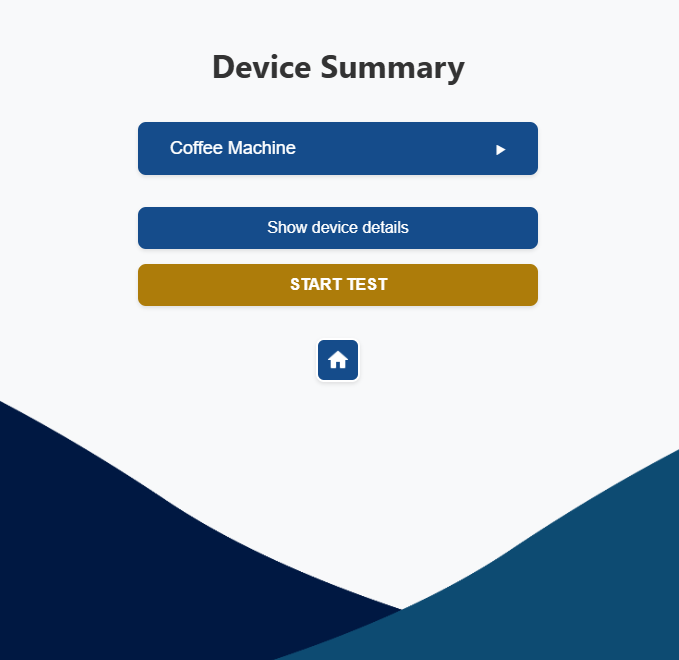
\includegraphics[width=.6\linewidth]{../../../Assets/Applicazione/DeviceSummary.png}
              \caption{Schermata di riepilogo}
        \end{figure}
      \end{center}
      \subsubsection{Visualizzazione degli asset}
        È presente un elemento cliccabile contenente il nome del dispositivo inserito; selezionandolo, viene visualizzata la \textit{lista}\textsubscript{\href{https://atlasteam9.github.io/Atlas/glossario.html\#Lista}{G}} di tutti gli asset del dispositivo. Ogni asset è rappresentato da un riquadro che mostra il nome e il tipo dell'asset.
        \begin{center}
        \begin{figure}[H]
              \centering
              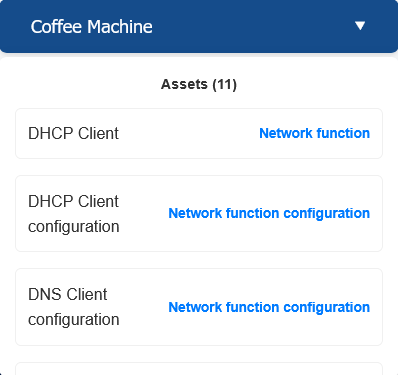
\includegraphics[scale=0.65]{../../../Assets/Applicazione/Assets.png}
              \caption{Lista degli asset}
        \end{figure}
      \end{center}
      \subsubsection{Visualizzazione dei dettagli degli asset}
        Premendo su un singolo asset nella \textit{lista}\textsubscript{\href{https://atlasteam9.github.io/Atlas/glossario.html\#Lista}{G}} degli asset, vengono visualizzati sullo schermo i suoi dettagli.
        \begin{center}
        \begin{figure}[H]
              \centering
              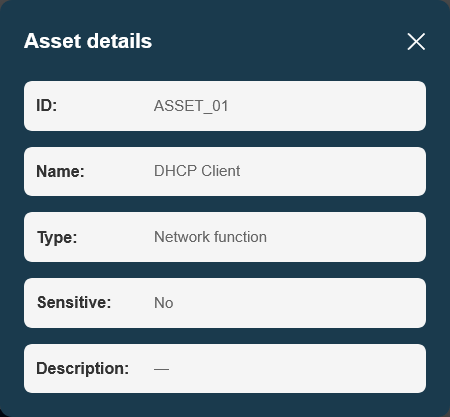
\includegraphics[width=.6\linewidth]{../../../Assets/Applicazione/Description.png}
              \caption{Descrizione di un asset}
              \label{fig:Asset}
        \end{figure}
      \end{center}
      Vengono descritte le principali caratteristiche dell'asset:
      \begin{itemize}
      \item \textbf{ID} : il codice identificativo dell'asset;
      \item \textbf{Name} : il nome dell'asset;
      \item \textbf{Type} : il tipo di asset;
      \item \textbf{Sensitive} : se l'asset è sensibile o meno;
      \item \textbf{Description} : la descrizione dell'asset.
      \end{itemize}

      \subsubsection{Visualizzazione dei dettagli del dispositivo}
      È possibile, inoltre, vedere tutti i dettagli di un dispositivo. Il bottone \textbf{Show Device Details} mostra a schermo la \textit{lista}\textsubscript{\href{https://atlasteam9.github.io/Atlas/glossario.html\#Lista}{G}} degli attributi del dispostivo.
      \begin{center}
        \begin{figure}[H]
              \centering
              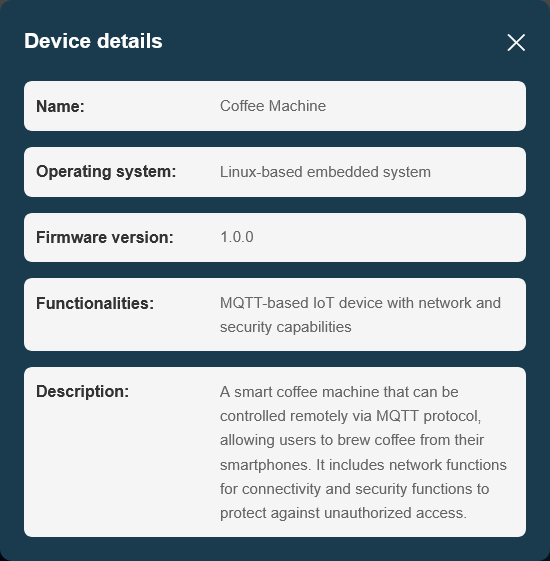
\includegraphics[width=.6\linewidth]{../../../Assets/Applicazione/DeviceDetails .png}
              \caption{Descrizione di un dispositivo}
              \label{fig:Descrizione}
        \end{figure}
      \end{center}
      In questa schermata è possibile vedere:
      \begin{itemize}
          \item \textbf{Name} : il nome del dispositivo;
          \item \textbf{Operating system} : il sistema operativo che usa il dispositivo;
          \item \textbf{Firmware version} : la versione del \textit{firmware}\textsubscript{\href{https://atlasteam9.github.io/Atlas/glossario.html\#Firmware}{G}} del dispositivo;
          \item \textbf{Functionalities} : tutte le funzionalità del dispositivo;
          \item \textbf{Description} : una descrizione del dispositivo.
      \end{itemize}
      \subsection{Avvio dei test}
      Dalla schermata di riepilogo è possibile avviare i test del dispositivo. Tutti gli asset vengono verificati tramite una serie di domande a risposta sì/no. È possibile navigare avanti o indietro tra le domande in base alle risposte fornite, e, in alto a sinistra, viene visualizzata la percentuale di completamento del test. Per salvare la sessione attuale, è possibile premere il pulsante Save and Exit, che salva la sessione in formato JSON e ti porta alla home. Per tornare alla schermata principale senza salvare, invece, si può premere il pulsante Home, situato in basso. Si procede rispondendo alle domande fino al completamento del test. 
      \begin{center}
        \begin{figure}[H]
              \centering
              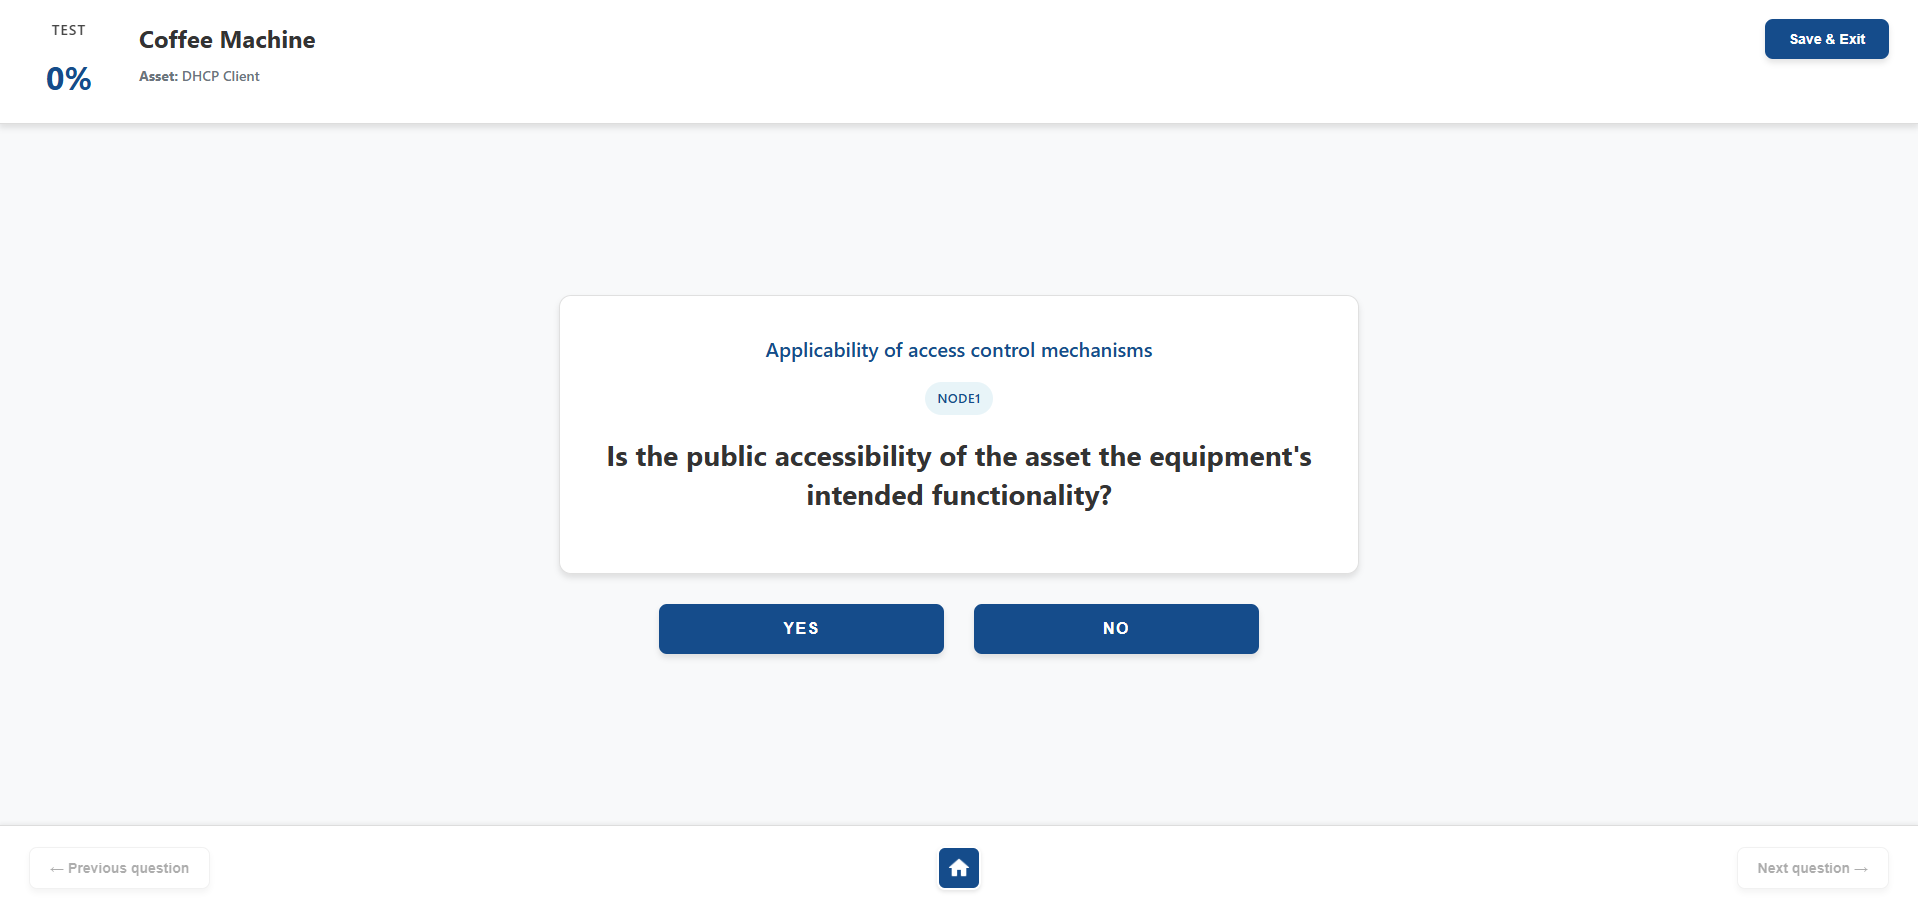
\includegraphics[width=.9\linewidth]{../../../Assets/Applicazione/Testing.png}
              \caption{Test in corso}
        \end{figure}
      \end{center}
      \subsection{Visualizzazione esito test}
        Al termine del test, per ogni \textit{requisito}\textsubscript{\href{https://atlasteam9.github.io/Atlas/glossario.html\#Requisito}{G}} viene visualizzato sullo schermo l'esito. Gli esiti possono essere di quattro tipi: 
      \begin{itemize}
          \item \textbf{PASS}: per tutti gli asset del dispositivo il \textit{requisito}\textsubscript{\href{https://atlasteam9.github.io/Atlas/glossario.html\#Requisito}{G}} è soddisfatto oppure in stato NON APPLICABILE. Tale \textit{requisito}\textsubscript{\href{https://atlasteam9.github.io/Atlas/glossario.html\#Requisito}{G}} quindi è soddisfatto per il dispositivo.
          \item \textbf{FAIL}: per tutti gli asset del dispositivo il \textit{requisito}\textsubscript{\href{https://atlasteam9.github.io/Atlas/glossario.html\#Requisito}{G}} è non soddisfatto oppure in stato NON APPLICABILE. Tale \textit{requisito}\textsubscript{\href{https://atlasteam9.github.io/Atlas/glossario.html\#Requisito}{G}} quindi non è soddisfatto per il dispositivo.
          \item \textbf{NOT APPLICABLE}: per tutti gli asset del dispositivo il \textit{requisito}\textsubscript{\href{https://atlasteam9.github.io/Atlas/glossario.html\#Requisito}{G}} è in stato NON APPLICABILE. Tale \textit{requisito}\textsubscript{\href{https://atlasteam9.github.io/Atlas/glossario.html\#Requisito}{G}} quindi non è applicabile al dispositivo.
          \item \textbf{NOT COMPLETED}: il test non è stato completato e quindi non sono disponibili risultati per il requisito. Questo stato può comparire se l'utente ha interrotto il test mentre era in corso e successivamente ha ricaricato la sessione.
      \end{itemize}
      Il dispositivo soggetto al test viene considerato conforme alla normativa \textit{EN 18031}\textsubscript{\href{https://atlasteam9.github.io/Atlas/glossario.html\#EN18031}{G}} se tutti i requisiti sono soddisfatti o non applicabili. Se invece è presente almeno un \textit{requisito}\textsubscript{\href{https://atlasteam9.github.io/Atlas/glossario.html\#Requisito}{G}} non soddisfatto, il dispositivo viene considerato non conforme.
       \begin{center}
        \begin{figure}[H]
              \centering
              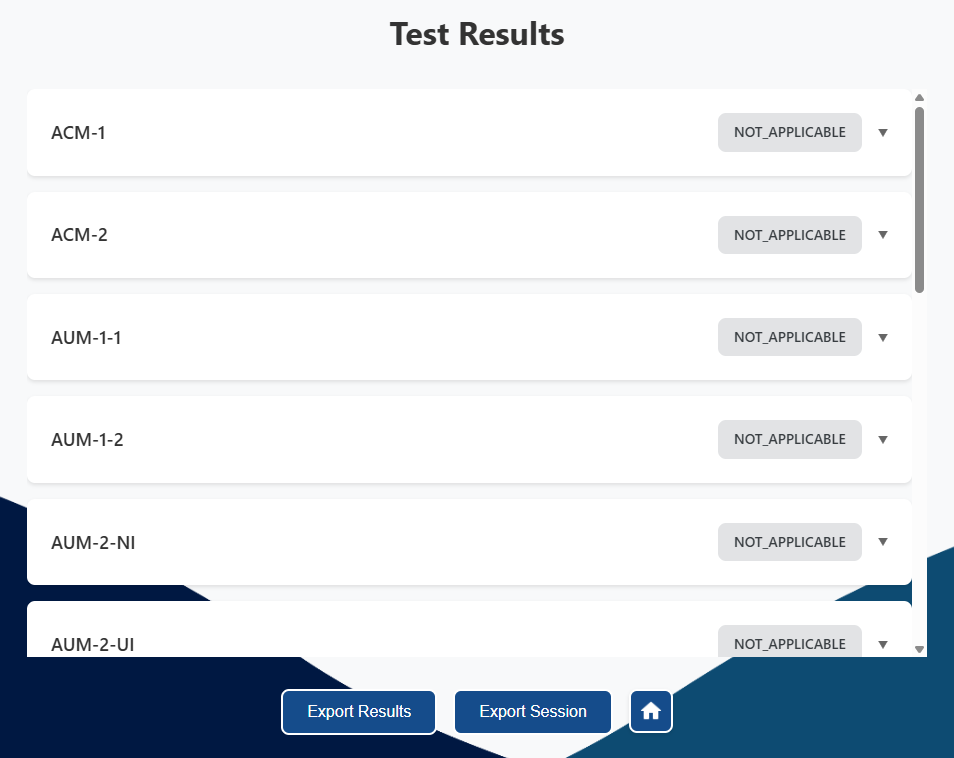
\includegraphics[width=.8\linewidth]{../../../Assets/Applicazione/TestResults.png}
              \caption{Esito dei test}
        \end{figure}
      \end{center}

        Per ognuno dei requisiti della \textit{norma}\textsubscript{\href{https://atlasteam9.github.io/Atlas/glossario.html\#Norma}{G}} è possibile, selezionando il box corrispondente, visionare la \textit{lista}\textsubscript{\href{https://atlasteam9.github.io/Atlas/glossario.html\#Lista}{G}} dei risultati dei singoli asset associati al requsito. 

        \begin{center}
            \begin{figure}[H]
                  \centering
                  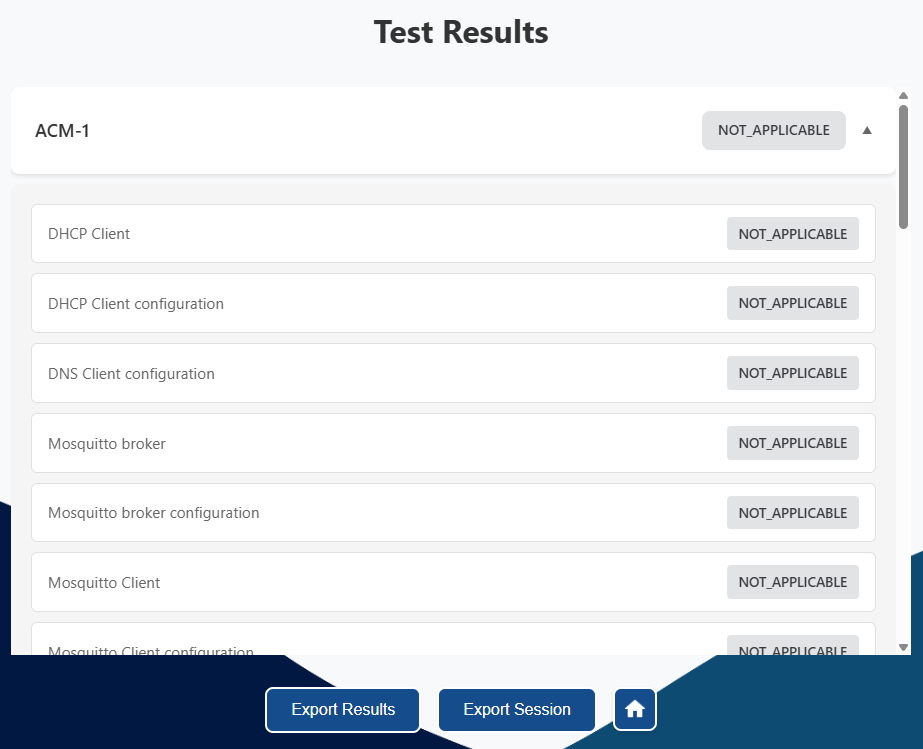
\includegraphics[width=.7\linewidth]{../../../Assets/Applicazione/TestAssetsResult.png}
                  \caption{Lista risultati assets}
            \end{figure}
        \end{center}
        
        Gli esiti dei test possono essere esportati mediante il pulsante \textbf{Export Results} in due formati: \textit{PDF}\textsubscript{\href{https://atlasteam9.github.io/Atlas/glossario.html\#PDF}{G}} e \textit{CSV}\textsubscript{\href{https://atlasteam9.github.io/Atlas/glossario.html\#CSV}{G}}. Anche la sessione può essere esportata mediante il pulsante \textbf{Export Session}, in formato JSON. Se esportati in formato \textit{PDF}\textsubscript{\href{https://atlasteam9.github.io/Atlas/glossario.html\#PDF}{G}}, gli esiti vengono visualizzati in forma tabellare.
        \begin{center}
        \begin{figure}[H]
              \centering
              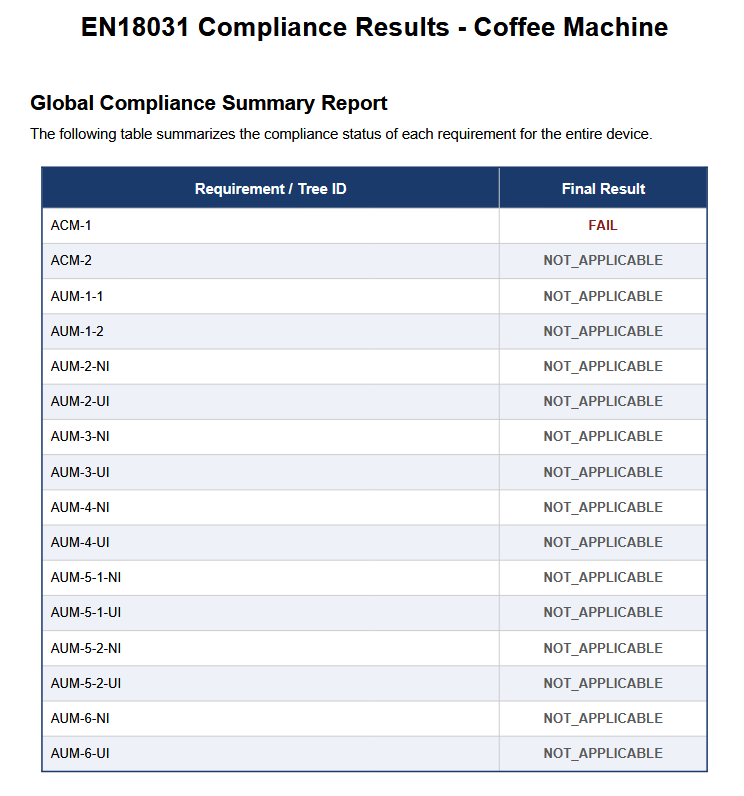
\includegraphics[width=.7\linewidth]{../../../Assets/Applicazione/PDFTest.png}
              \caption{Esito esportato come PDF}
        \end{figure}
      \end{center}
      \subsection{Creazione di un dispositivo}
      Per creare un nuovo dispositivo, occorre premere il pulsante \textbf{Create New Device} che si trova nella homepage della web-app. Una volta premuto il pulsante, viene visualizzato un modulo di compilazione, in cui è possibile inserire i dati relativi al dispositivo. I dati da inserire sono riferiti nella figura \ref{fig:Descrizione}. 
       \begin{center}
        \begin{figure}[H]
              \centering
              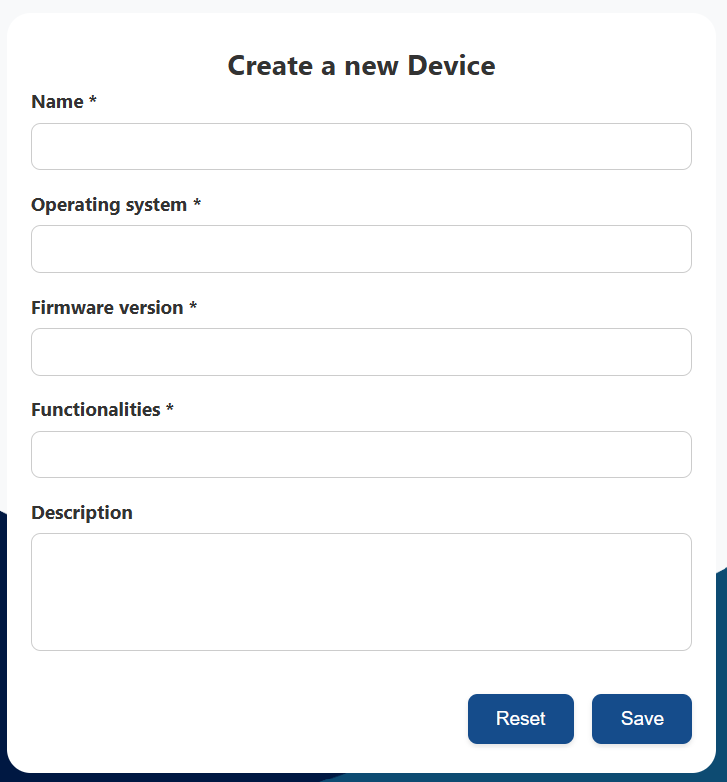
\includegraphics[width=.7\linewidth]{../../../Assets/Applicazione/CreateDevice .png}
              \caption{Creazione di un dispositivo}
        \end{figure}
      \end{center}
      \subsubsection{Creazione di un asset}
      Dopo la creazione di un dispositivo, l'utente viene portato alla schermata di gestione degli asset. Azionando il pulsante \textbf{Add new asset}, è possibile creare dei nuovi asset associati al dispositivo. La fase di creazione prevede la compilazione di un modulo, in cui è possibile:
      \begin{itemize}
        \item inserire il campo Name,
        \item selezionare il campo Type da una \textit{lista}\textsubscript{\href{https://atlasteam9.github.io/Atlas/glossario.html\#Lista}{G}} di opzioni predefinite,
        \item selezionare il campo Is Sensitive tramite un toggle,
        \item inserire opzionalmente il campo Description.
      \end{itemize}
      \begin{center}
        \begin{figure}[H]
              \centering
              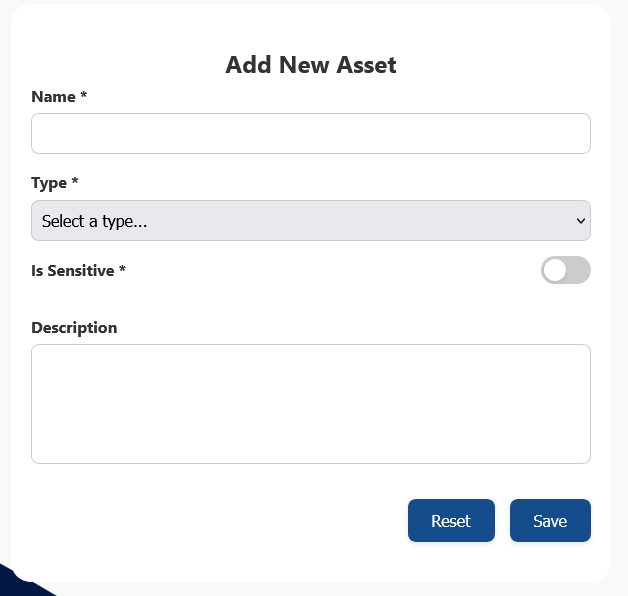
\includegraphics[width=.6\linewidth]{../../../Assets/Applicazione/AssetCreate.png}
              \caption{Creazione asset}
        \end{figure}
      \end{center}
      Dopo aver creato un nuovo asset, questo viene visualizzato nella \textit{lista}\textsubscript{\href{https://atlasteam9.github.io/Atlas/glossario.html\#Lista}{G}} degli asset nella schermata di gestione. Inoltre, è possibile eliminare un asset creato premendo il pulsante con l'icona di un cestino, situato accanto all'asset nella lista. L'utente può tornare alla schermata di riepilogo premendo il pulsante
      \textbf{Go to summary}.
      \begin{center}
        \begin{figure}[H]
              \centering
              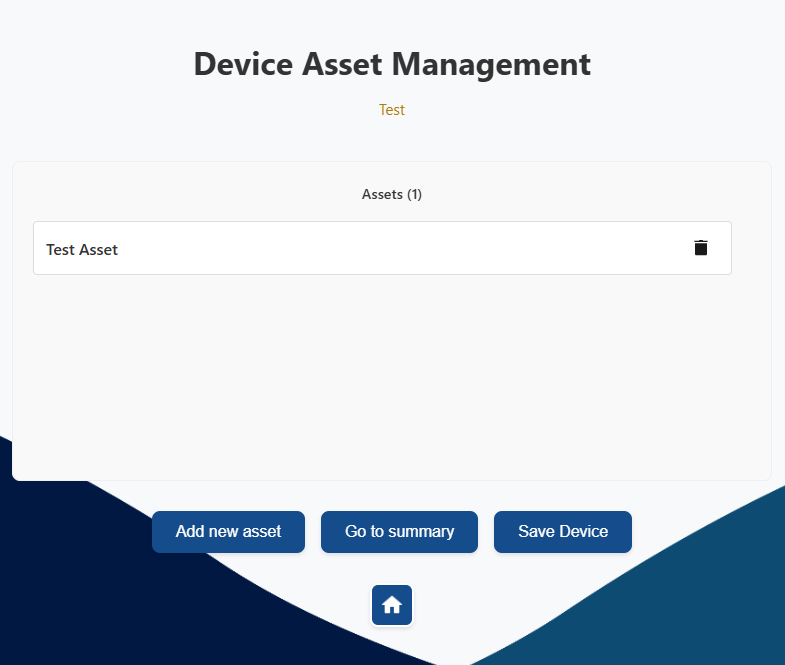
\includegraphics[width=.65\linewidth]{../../../Assets/Applicazione/AssetManager.png}
              \caption{Gestione asset}
        \end{figure}
      \end{center}
      
      \subsubsection{Salvataggio di un dispositivo}
      Completata la creazione degli asset, è possibile salvare il dispositivo in formato JSON premendo il pulsante \textbf{Save Device}. Il salvataggio è consentito solo se il dispositivo contiene almeno un asset.

      Se prima di andare alla schermata successiva non viene selezionato il pulsante \textbf{Save Device}, a schermo compare un messaggio che avvisa l'utente della presenza di modifiche al dispositivo non salvate. Se si clicca "YES" il dispositivo viene salvato in formato JSON nel pc dell'utente altrimenti si passa direttamente alla schemata "Device Summary" e le modifiche al dispositivo non verranno salvate. 

      \begin{center}
        \begin{figure}[H]
              \centering
              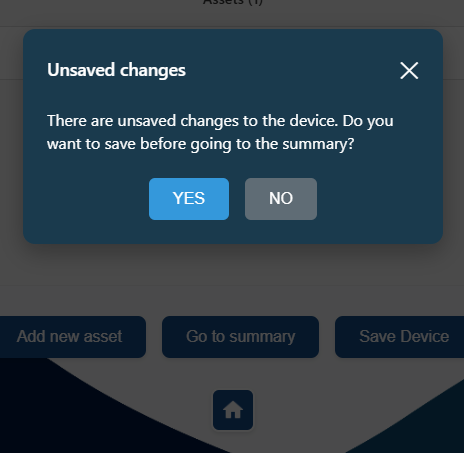
\includegraphics[width=.4\linewidth]{../../../Assets/Applicazione/ModificheDispositivoNonSalvate.png}
              \caption{Modifiche non salvate}
        \end{figure}
      \end{center}

      \subsection{Ripresa di una sessione non completata}
      L'applicazione consente la ripresa di una sessione precedentemente salvata dall'utente. La ripresa si ottiene premendo il pulsante \textbf{Upload previous session} che si trova nella homepage. Successivamente, viene visualizzata una finestra di selezione file. Gli unici file ammessi sono i file di tipo JSON conformi al file di sessione previsto per l'applicazione.
      Una volta selezionato il file, l'utente viene portato alla schermata degli esiti del test non completato.
      \begin{center}
        \begin{figure}[H]
              \centering
              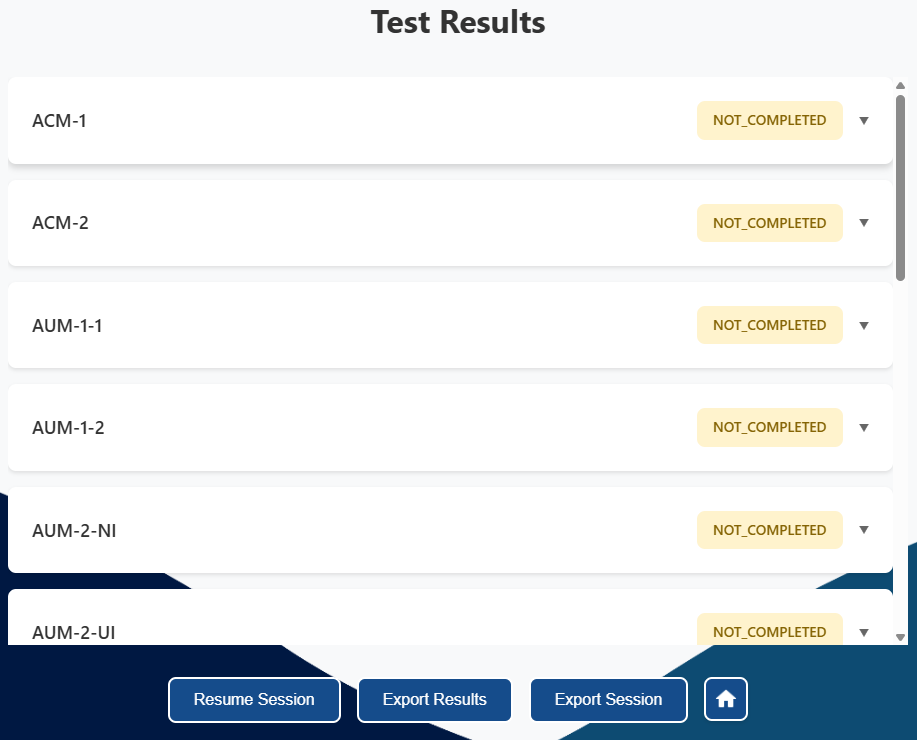
\includegraphics[width=.6\linewidth]{../../../Assets/Applicazione/UploadSessionResult.png}
              \caption{Ripresa di una sessione non completata}
        \end{figure}
      \end{center}
      La schermata è simile a quella degli esiti dei test, ma in questo caso l'utente può riprendere i test dal punto in cui si era interrotto l'ultima volta azionando il pulsante \textbf{Resume Session}.

      \subsection{Modifica di una sessione completata}
      L'applicazione consente anche la modifica di una sessione precedentemente finita e salvata dall'utente. La modifica si ottiene premendo il pulsante \textbf{Upload previous session} che si trova nella homepage. Successivamente, viene visualizzata una finestra di selezione file. Gli unici file ammessi sono i file di tipo JSON conformi al file di sessione previsto per l'applicazione.
      Una volta selezionato il file, l'utente viene portato alla schermata degli esiti dei test.
      \begin{center}
        \begin{figure}[H]
              \centering
              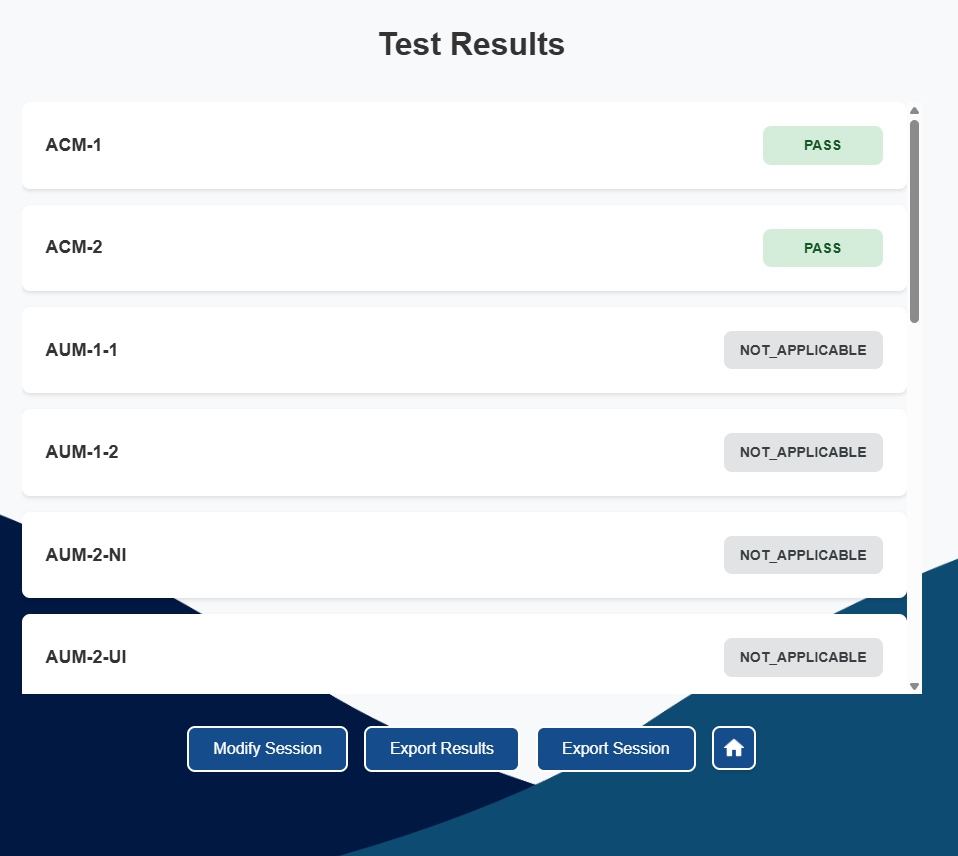
\includegraphics[scale=0.45]{../../../Assets/Applicazione/RipresaSessioneCompletata.png}
              \caption{Ripresa di una sessione completata}
        \end{figure}
      \end{center}
      La schermata è simile a quella degli esiti dei test, ma in questo caso l'utente può andare alla schermata di modifica dei risultati azionando il pulsante  \textbf{Modify Session}.

      \subsection{Pagina requisiti modificabili}
      Una volta selezionato il pulsante \textbf{Modify Session} viene visualizzata la pagina di modifica con al suo interno la \textit{lista}\textsubscript{\href{https://atlasteam9.github.io/Atlas/glossario.html\#Lista}{G}} dei soli requisiti modificabili.
      \begin{center}
        \begin{figure}[H]
              \centering
              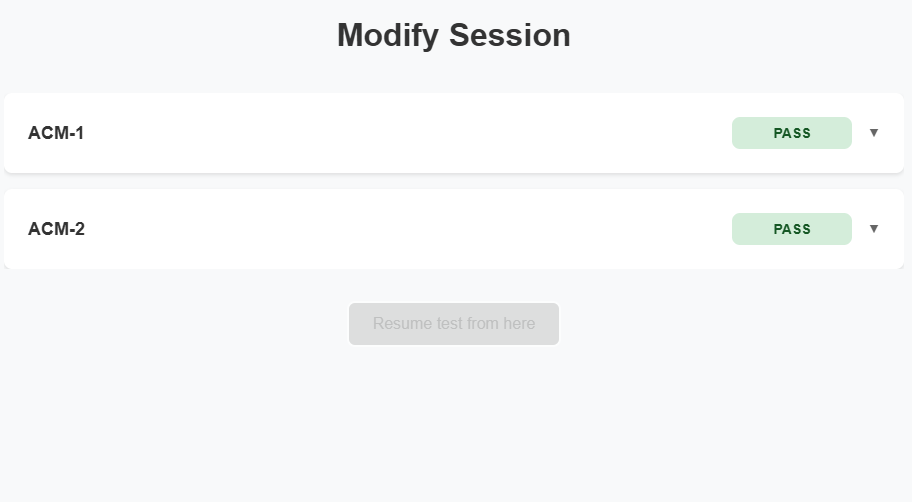
\includegraphics[scale=0.45]{../../../Assets/Applicazione/SchermataModificaSessione.png}
              \caption{Modifica di un test}
        \end{figure}
      \end{center}

      \subsection{Visualizzazione asset modificabili}
      Per iniziare la modifica bisogna selezionare un asset specifico. Per visualizzare gli asset da cui è possibile modificare bisogna cliccare sul box corrispondente ad un requisito. Una volta cliccato si apre la \textit{lista}\textsubscript{\href{https://atlasteam9.github.io/Atlas/glossario.html\#Lista}{G}} degli asset da cui è possibile far ripartire l'esecuzione del test. 
      \begin{center}
        \begin{figure}[H]
              \centering
              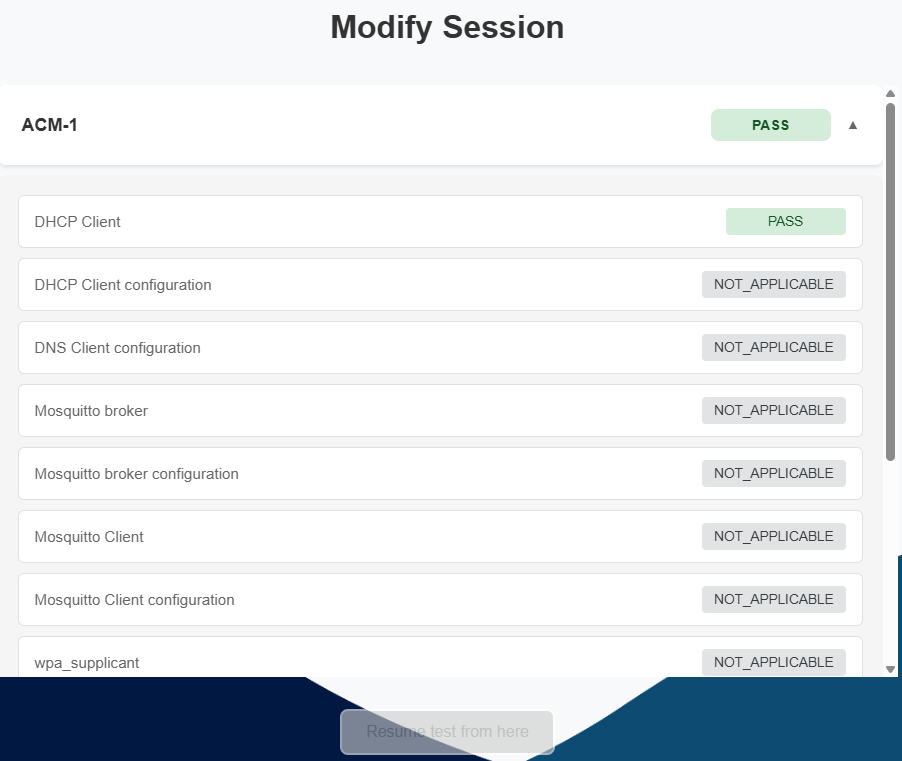
\includegraphics[scale=0.5]{../../../Assets/Applicazione/VisualizzazioneAssetModificabili.png}
              \caption{Visualizzazione asset modificabili}
        \end{figure}
      \end{center}

      \subsection{Modifica del test}
      Se si clicca su un asset modificabile questo viene evidenziato. Allo stesso modo diventa cliccabile il pulsante in fondo alla pagina che permette di riprendere il test da quel preciso asset partendo dal \textit{requisito}\textsubscript{\href{https://atlasteam9.github.io/Atlas/glossario.html\#Requisito}{G}} di cui faceva parte.
      \begin{center}
        \begin{figure}[H]
              \centering
              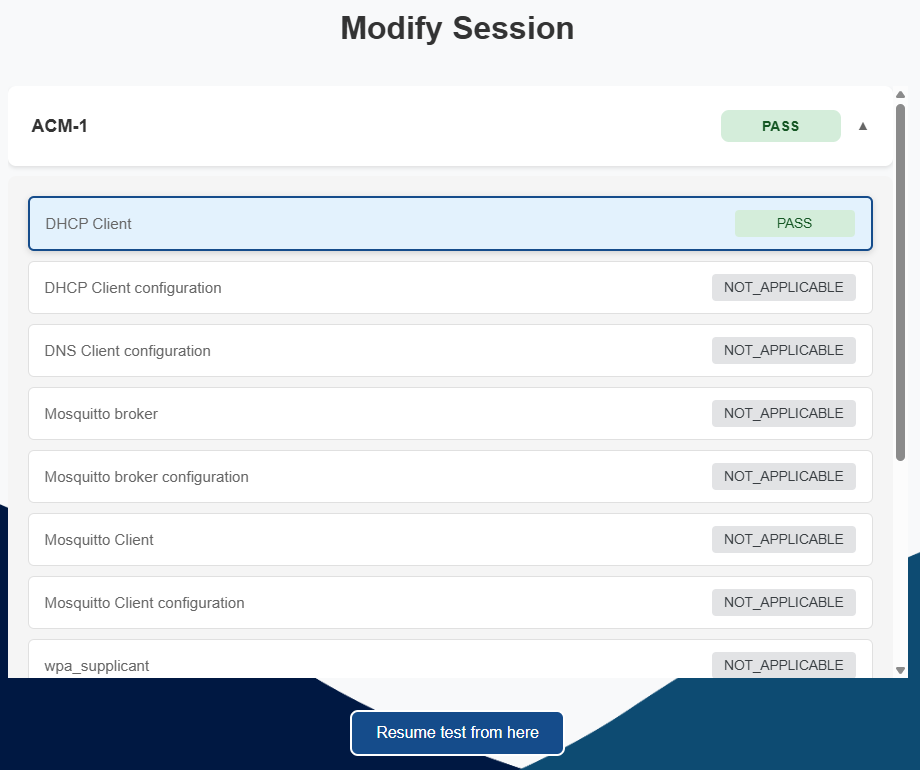
\includegraphics[scale=0.5]{../../../Assets/Applicazione/ModificaTest.png}
              \caption{Modifica test}
        \end{figure}
      \end{center}

      Una volta cliccato il pulsante \textbf{Resume test from here} la schermata è identica a quella dell'esecuzione del test. In questo caso però il test parte da un punto specifico selezionato dall'utente e non dall'inizio. 

    \subsection{Asset non modificabili}
        Se viene caricata una sessione che include asset con esito NOT APPLICABLE, questi potrebbero non essere modificabili, in quanto potrebbero dipendere da altri asset anch'essi con esito NOT APPLICABLE. Per poter modificare un test, è necessario ripartire da un asset che non abbia dipendenze NOT APPLICABLE. 
            \begin{center}
        \begin{figure}[H]
              \centering
              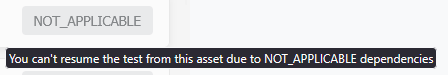
\includegraphics[scale=0.7]{../../../Assets/Applicazione/NonModificabile.png}
              \caption{Asset non modificabile}
        \end{figure}
      \end{center}
    \subsection{Domande non recuperabili}
    Se si modifica una risposta precedente, non sarà più possibile proseguire con le domande premendo il pulsante \textbf{Next Question}; sarà invece necessario rispondere nuovamente alle domande. Ciò è dovuto al fatto che i risultati vengono salvati in tempo reale. Il pulsante \textbf{Next Question} rimarrà disabilitato.
     \begin{center}
        \begin{figure}[H]
              \centering
              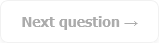
\includegraphics[scale=0.5]{../../../Assets/Applicazione/NextDisabled.png}
              \caption{Pulsante Next Question disabilitato}
        \end{figure}
      \end{center}
    \subsection{Possibili errori}
     Questa sezione elenca alcuni errori che l'utente potrebbe incontrare durante l'utilizzo dell'applicazione e fornisce indicazioni su come risolverli.
     \subsubsection{Errore nel caricamento di un dispositivo}
    Questo \textit{errore}\textsubscript{\href{https://atlasteam9.github.io/Atlas/glossario.html\#Errore}{G}} è accompagnato dal codice 422 e indica che il file JSON del dispositivo è formattato in modo errato e quindi non può essere letto dal sistema. Questo \textit{errore}\textsubscript{\href{https://atlasteam9.github.io/Atlas/glossario.html\#Errore}{G}} può verificarsi se nel file JSON ci sono errori di battitura durante la compilazione manuale, oppure se viene caricato un file non compatibile con l'applicazione.
    \begin{center}
        \begin{figure}[H]
              \centering
              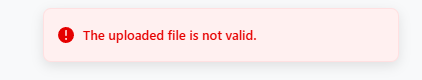
\includegraphics[scale=0.6]{../../../Assets/Applicazione/ErroreFile.png}
              \caption{Errore caricamento dispositivo}
        \end{figure}
      \end{center}
      \subsubsection{Errore compilazione modulo}
     Questo \textit{errore}\textsubscript{\href{https://atlasteam9.github.io/Atlas/glossario.html\#Errore}{G}} si verifica quando non vengono compilati tutti i campi obbligatori. L'applicazione segnala immediatamente all'utente il campo da completare.
     \begin{center}
        \begin{figure}[H]
              \centering
              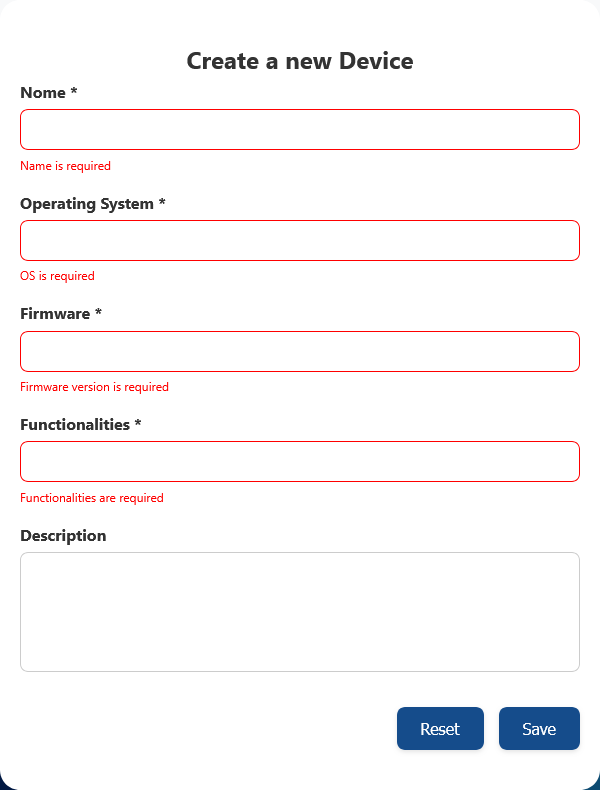
\includegraphics[scale=0.26]{../../../Assets/Applicazione/ErrorForm.png}
              \caption{Errore mancata compilazione}
        \end{figure}
      \end{center}
      Questo \textit{errore}\textsubscript{\href{https://atlasteam9.github.io/Atlas/glossario.html\#Errore}{G}} può verificarsi durante la creazione di un nuovo dispositivo oppure nella creazione di un nuovo asset.
      \subsubsection{Errore server irraggiungibile}
      Questo \textit{errore}\textsubscript{\href{https://atlasteam9.github.io/Atlas/glossario.html\#Errore}{G}} si verifica quando il backend della web app non è attivo oppure quando l'URL presente nel file .env è diverso da quello predefinito. Se l'URL è diverso, scaricare nuovamente il file .env e sostituire quello attualmente presente nei file.
      \begin{center}
        \begin{figure}[H]
              \centering
              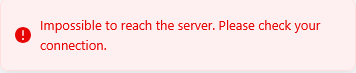
\includegraphics[scale=0.58]{../../../Assets/Applicazione/ServerError.png}
              \caption{Errore server irraggiungibile}
        \end{figure}
      \end{center}
      
      \subsubsection{Errore nell'invio della risposta}
        Durante l'utilizzo dell'applicazione può verificarsi un \textit{errore}\textsubscript{\href{https://atlasteam9.github.io/Atlas/glossario.html\#Errore}{G}} nel caso in cui la stessa sessione venga aperta contemporaneamente in più schede del browser. Ad \textit{esempio}\textsubscript{\href{https://atlasteam9.github.io/Atlas/glossario.html\#Esempio}{G}}, un utente apre una sessione incompleta in una prima scheda e seleziona il pulsante \textbf{Modify Session}. Successivamente, apre una seconda scheda del browser, carica lo stesso file di sessione e, dopo aver premuto nuovamente \textbf{Modify Session}, torna alla schermata principale tramite il pulsante Home. Tornando alla prima scheda e tentando di proseguire il test selezionando YES o NO, viene visualizzato un messaggio di \textit{errore}\textsubscript{\href{https://atlasteam9.github.io/Atlas/glossario.html\#Errore}{G}} “Failed to submit answer.” Ciò accade perché tornando alla home dalla seconda scheda la sessione viene eliminata localmente e quindi non è più possibile proseguire con la prima scheda. Per risolvere questo problema, è necessario evitare di aprire la stessa sessione in più schede del browser.
        \begin{center}
        \begin{figure}[H]
              \centering
              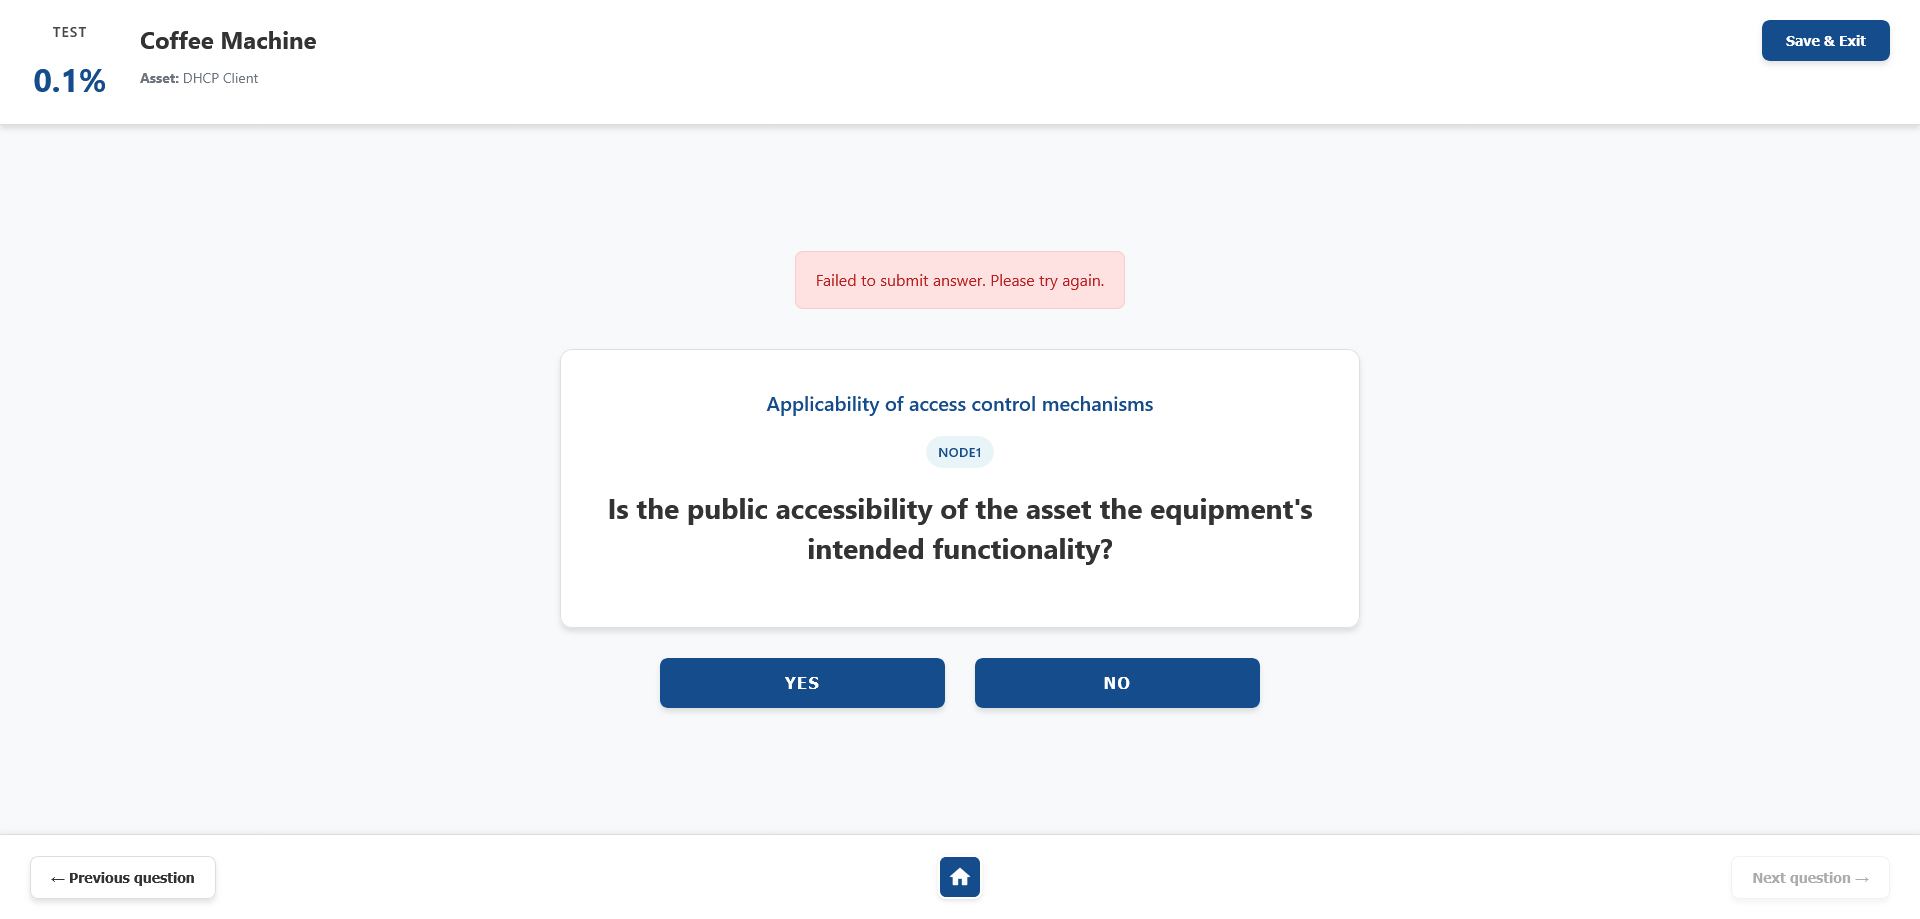
\includegraphics[scale=0.25]{../../../Assets/Applicazione/ErrorTabs.png}
              \caption{Errore risposta}
        \end{figure}
      \end{center}
      \subsubsection{Impossibile recuperare l'immagine}
      L'\textit{errore}\textsubscript{\href{https://atlasteam9.github.io/Atlas/glossario.html\#Errore}{G}} \textbf{"Failed to connect to the docker API at npipe:\newline////./pipe/dockerDesktopLinuxEngine; check if the path is correct and if the \newline daemon is running:"} si verifica quando si tenta di creare l'immagine \textit{Docker}\textsubscript{\href{https://atlasteam9.github.io/Atlas/glossario.html\#Docker}{G}} tramite terminale, ma il \textit{Docker}\textsubscript{\href{https://atlasteam9.github.io/Atlas/glossario.html\#Docker}{G}} Engine non è attivo. Per risolverlo, avviare \textit{Docker}\textsubscript{\href{https://atlasteam9.github.io/Atlas/glossario.html\#Docker}{G}} Engine. Se si è da Windows o Mac, avviare \textit{Docker}\textsubscript{\href{https://atlasteam9.github.io/Atlas/glossario.html\#Docker}{G}} Desktop.
      \subsection{Supporto tecnico}
      In caso di situazioni estreme o anomalie, è possibile contattare il team scrivendo all'indirizzo email  \textbf{team9.atlas@gmail.com} e descrivendo il problema riscontrato.
\end{document}            